\section{Pendahuluan}
\subsection{Latar Belakang}
Pada era saat ini tidak bisa dipungkiri lagi bahwa perangkat elektronik yang kita gunakan sehari-hari saling berhubungan dengan satu sama lain dan menciptakan sebuah jaringan perangkat komputer. Skala dari jaringan komputer ini pun sudah semakin besar,mulai dari jaringan skala kecil seperti antar perangkat pribadi, maupun seluas antar negara dan benua seperti internet. Selain itu, metode penghubungan antar perangkat tidak lagi terbatas secara fisik dengan teknologi wireless, dan apabila diinginkan penghubungan secara fisik maka sekarang terdapat pilihan kabel yang dapat mentransfer data lebih cepat seperti \textit{fiber optic}.\\
Pada Modul 1 praktikum jaringan komputer ini membahas tentang crimping kabel dan Routing IPv4 bertujuan untuk meningkatkan pemahaman mahasiswa terhadap dasar dari pembuatan jaringan komputer yaitu melakukan penentuan IP perangkat komputer dan melakukan routing, serta memberikan pengetahuan tentang tahap dasar pembuatan jaringan komputer dengan kabel yaitu crimping kabel. 
\subsection{Dasar Teori}
Jaringan Komputer adalah sebuah sistem yang menghubungkan 2 atau lebih perangkat komputer yang dibuat agar perangkat-perangkat tersebut dapat bertukar informasi dan sumber daya. Berdasarkan skalanya jaringan komputer dibagi menjadi 5, yaitu Personal Area Network (PAN), Local Area Network (LAN), Campus Area Network (CAN), Metropolitan Area Network (MAN), dan Wide Area Network (WAN). Seiring berkembangnya zaman, jaringan komputer saat ini dapat dibuat baik secara fisik menggunakan kabel sebagai perantaranya ataupun secara wireless dengan menggunakan gelombang radio untuk perantaranya. Kedua metode pembangunan jaringan ini tentunya memiliki keuntungan dan kerugiannya tersendiri, seperti wireless yang jauh lebih bebas dan lebih murah dibanding jaringan dengan kabel, namun jaringan dengan kabel bisa lebih cepat dan lebih aman dibandingkan wireless yang membuat jaringan dengan kabel menjadi pilihan yang cocok untuk penggunaan dikantor atau sejenisnya. Jenis kabel yang biasanya digunakan untuk membuat jaringan komputer adalah kabel jenis UTP(Unshielded Twisted Pair), dimana didalam kabel UTP terdapat kumpulan kabel dengan berbagai warna yang memiliki kode fungsinya masing-masing, seperti kabel putih-oranye yang berfungsi untuk transmit Data dan putih-hijau untuk receive data. Untuk menggunakan kabel untuk membangun jaringan komputer perlu dilakukan proses yang disebut dengan \textit{crimping} yaitu proses penyambungan kabel dengan konektor RJ-45. Untuk proses \textit{crimping} ini terdapat 2 kombinasi konfigurasi yaitu T586A dan T586B. Kemudian untuk metode penghubungan dibagi menjadi Straight-Through yang digunakan untuk menghubungkan perangkat seperti komputer, terminal, dan printer dengan perangkat seperti switch, router, dan modem serta metode Crossover yang digunakan untuk menghubungkan 2 perangkat yang sama seperti komputer dengan komputer, router dengan router, dsb. \\
Untuk dapat melakukan pertukaran informasi maka perangkat komputer membutuhkan sebuah tanda pengenal yang membedakan perangkat tersebut dengan perangkat lainnya dalam sebuah jaringan komputer, penanda ini yang kita sebut dengan IP Address. IP Address sendiri dapat dibagi menjadi Dynamic IP Address dan Static IP Address. Dynamic IP Address adalah alamat IP yang dapat berubah secara otomatis, biasanya diberikan oleh ISP ketika perangkat terhubung ke internet. Keuntungan dari IP dinamis adalah hacker tidak akan dengan mudah mengakses perangkat. Sementara Static IP Address adalah alamat IP yang tetap, penggunaannya lebih cocok untuk server web atau penggunaan lokal dan terisolasi. Saat ini, versi alamat IP yang paling sering digunakan adalah IPv4. Versi IP ini menggunakan angka 32-bit yang dibagi menjadi 4 kelompok, sehingga setiap kelompok memiliki 8-bit. Cara penulisan dari IPv4 adalah xxx.xxx.xxx.xxx dimana setiap kelompok angka dapat diisi dari 0 hingga 255. Proses penambahan IP Address sebuah perangkat kedalam sebuah jaringan disebut dengan Routing. Metode routing sendiri dibagi menjadi Static Routing dan Dynamic Routing. 
%===========================================================%
\section{Tugas Pendahuluan}
Bagian ini berisi jawaban dari tugas pendahuluan yang telah anda kerjakan, beserta penjelasan dari jawaban tersebut
\begin{enumerate}
	\item $\bullet$ Departemen Produksi: 192.168.10.0/26\\
	Rentang IP Host: 192.168.10.1/26 - 192.168.10.63/26 \\
	$\bullet$ Departemen Administrasi: 192.168.10.64/27\\
	Rentang IP Host: 192.168.10.65/27 - 192.168.10.95/27\\
	$\bullet$ Departemen Keuangan: 192.168.10.96/28\\
	Rentang IP Host: 192.168.10.97/28 - 192.168.10.110\\
	$\bullet$ Departemen R \& D: 192.168.10.128/25\\
	Rentang IP Host: 192.168.10.129/25 - 192.168.10.255/25\\
	Total Subnet: 4\\
	\item 
		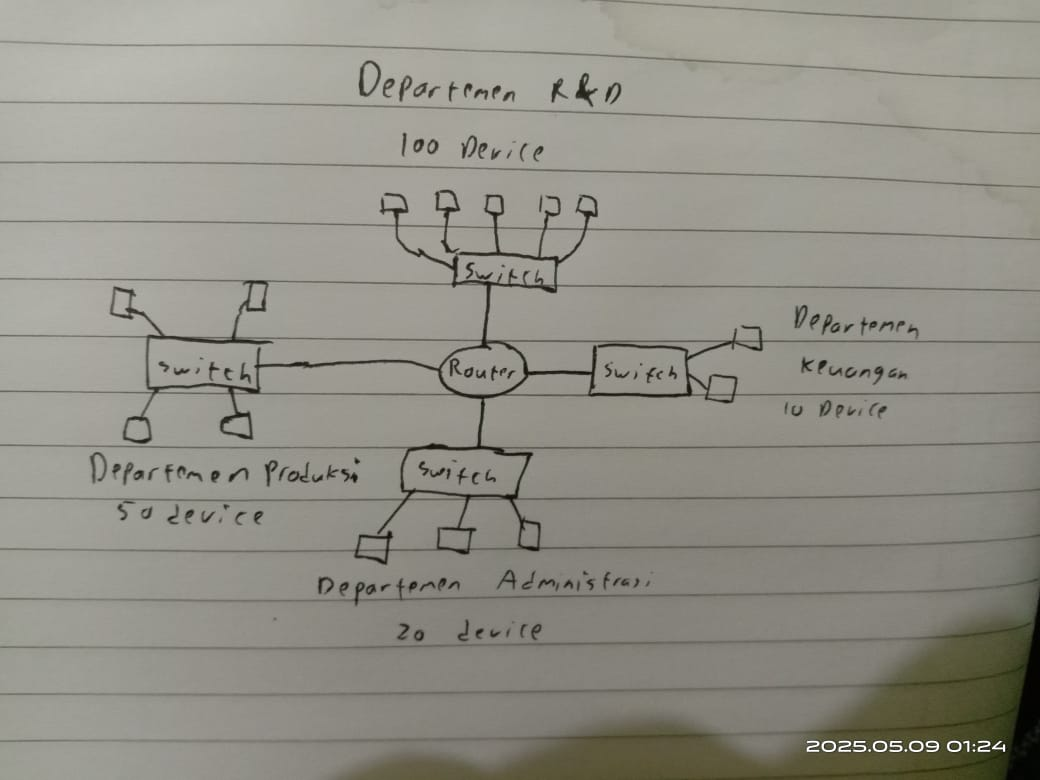
\includegraphics[width=0.5\textwidth]{"C:/Users/BINTANG/praktikum-jarkom/Template Laporan Sementara/P1/img/tugaspendahuluan-no2.jpg"}
	\item Tabel Router A\\
	\begin{tabular}{|l|c|l|l|}
		\hline
		\textbf{Destination} & \textbf{Prefix} & \textbf{Gateway} & \textbf{Interface Tujuan} \\
		\hline
		192.168.10.128   & /25 & -   & ke R\&D \\
		192.168.10.0      & /26  & -      & ke Produksi \\
		192.168.10.64    & /27 & -  & ke Administrasi \\
		192.168.10.96       & /28  & -   & ke Keuangan \\
		\hline
	\end{tabular}\\

	\item Menurut saya static routing adalah metode routing paling cocok untuk perusahaan ini. Karena untuk penggunaan lokal perusahaan tidak diperlukan perubahan jaringan terlalu sering, selain itu metode static routing mempermudah maintenance jaringan.
\end{enumerate}